\chapter{Bread and Salt}

Madame de Morcerf entered an archway of trees with her companion. It
led through a grove of lindens to a conservatory.

“It was too warm in the room, was it not, count?” she asked.

“Yes, madame; and it was an excellent idea of yours to open the doors
and the blinds.” As he ceased speaking, the count felt the hand of
Mercédès tremble. “But you,” he said, “with that light dress, and
without anything to cover you but that gauze scarf, perhaps you feel
cold?”

“Do you know where I am leading you?” said the countess, without
replying to the question.

“No, madame,” replied Monte Cristo; “but you see I make no resistance.”

“We are going to the greenhouse that you see at the other end of the
grove.”

The count looked at Mercédès as if to interrogate her, but she
continued to walk on in silence, and he refrained from speaking. They
reached the building, ornamented with magnificent fruits, which ripen
at the beginning of July in the artificial temperature which takes the
place of the sun, so frequently absent in our climate. The countess
left the arm of Monte Cristo, and gathered a bunch of Muscatel grapes.

“See, count,” she said, with a smile so sad in its expression that one
could almost detect the tears on her eyelids—“see, our French grapes
are not to be compared, I know, with yours of Sicily and Cyprus, but
you will make allowance for our northern sun.” The count bowed, but
stepped back.

“Do you refuse?” said Mercédès, in a tremulous voice.

“Pray excuse me, madame,” replied Monte Cristo, “but I never eat
Muscatel grapes.”

Mercédès let them fall, and sighed. A magnificent peach was hanging
against an adjoining wall, ripened by the same artificial heat.
Mercédès drew near, and plucked the fruit.

“Take this peach, then,” she said. The count again refused. “What,
again?” she exclaimed, in so plaintive an accent that it seemed to
stifle a sob; “really, you pain me.”

A long silence followed; the peach, like the grapes, fell to the
ground.

“Count,” added Mercédès with a supplicating glance, “there is a
beautiful Arabian custom, which makes eternal friends of those who have
together eaten bread and salt under the same roof.”

“I know it, madame,” replied the count; “but we are in France, and not
in Arabia, and in France eternal friendships are as rare as the custom
of dividing bread and salt with one another.”

“But,” said the countess, breathlessly, with her eyes fixed on Monte
Cristo, whose arm she convulsively pressed with both hands, “we are
friends, are we not?”

The count became pale as death, the blood rushed to his heart, and then
again rising, dyed his cheeks with crimson; his eyes swam like those of
a man suddenly dazzled.

“Certainly, we are friends,” he replied; “why should we not be?”

The answer was so little like the one Mercédès desired, that she turned
away to give vent to a sigh, which sounded more like a groan. “Thank
you,” she said. And they walked on again. They went the whole length of
the garden without uttering a word.

“Sir,” suddenly exclaimed the countess, after their walk had continued
ten minutes in silence, “is it true that you have seen so much,
travelled so far, and suffered so deeply?”

“I have suffered deeply, madame,” answered Monte Cristo.

“But now you are happy?”

“Doubtless,” replied the count, “since no one hears me complain.”

“And your present happiness, has it softened your heart?”

“My present happiness equals my past misery,” said the count.

“Are you not married?” asked the countess.

“I, married?” exclaimed Monte Cristo, shuddering; “who could have told
you so?”

“No one told me you were, but you have frequently been seen at the
Opera with a young and lovely woman.”

“She is a slave whom I bought at Constantinople, madame, the daughter
of a prince. I have adopted her as my daughter, having no one else to
love in the world.”

“You live alone, then?”

“I do.”

“You have no sister—no son—no father?”

“I have no one.”

“How can you exist thus without anyone to attach you to life?”

“It is not my fault, madame. At Malta, I loved a young girl, was on the
point of marrying her, when war came and carried me away. I thought she
loved me well enough to wait for me, and even to remain faithful to my
memory. When I returned she was married. This is the history of most
men who have passed twenty years of age. Perhaps my heart was weaker
than the hearts of most men, and I suffered more than they would have
done in my place; that is all.”

The countess stopped for a moment, as if gasping for breath. “Yes,” she
said, “and you have still preserved this love in your heart—one can
only love once—and did you ever see her again?”

\begin{figure}[ht]
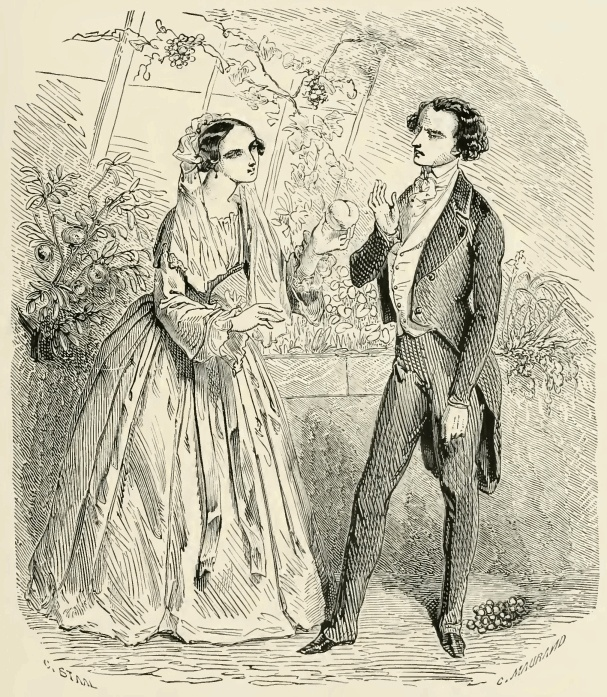
\includegraphics[width=\textwidth]{30309m.jpg}
\end{figure}

“Never.”

“Never?”

“I never returned to the country where she lived.”

“To Malta?”

“Yes; Malta.”

“She is, then, now at Malta?”

“I think so.”

“And have you forgiven her for all she has made you suffer?”

“Her,—yes.”

“But only her; do you then still hate those who separated you?”

“I hate them? Not at all; why should I?” The countess placed herself
before Monte Cristo, still holding in her hand a portion of the
perfumed grapes.

“Take some,” she said.

“Madame, I never eat Muscatel grapes,” replied Monte Cristo, as if the
subject had not been mentioned before. The countess dashed the grapes
into the nearest thicket, with a gesture of despair.

“Inflexible man!” she murmured. Monte Cristo remained as unmoved as if
the reproach had not been addressed to him.

Albert at this moment ran in. “Oh, mother,” he exclaimed, “such a
misfortune has happened!”

“What? What has happened?” asked the countess, as though awakening from
a sleep to the realities of life; “did you say a misfortune? Indeed, I
should expect misfortunes.”

“M. de Villefort is here.”

“Well?”

“He comes to fetch his wife and daughter.”

“Why so?”

“Because Madame de Saint-Méran is just arrived in Paris, bringing the
news of M. de Saint-Méran’s death, which took place on the first stage
after he left Marseilles. Madame de Villefort, who was in very good
spirits, would neither believe nor think of the misfortune, but
Mademoiselle Valentine, at the first words, guessed the whole truth,
notwithstanding all the precautions of her father; the blow struck her
like a thunderbolt, and she fell senseless.”

“And how was M. de Saint-Méran related to Mademoiselle de Villefort?”
said the count.

“He was her grandfather on the mother’s side. He was coming here to
hasten her marriage with Franz.”

“Ah, indeed!”

“So Franz must wait. Why was not M. de Saint-Méran also grandfather to
Mademoiselle Danglars?”

“Albert, Albert,” said Madame de Morcerf, in a tone of mild reproof,
“what are you saying? Ah, count, he esteems you so highly, tell him
that he has spoken amiss.”

And she took two or three steps forward. Monte Cristo watched her with
an air so thoughtful, and so full of affectionate admiration, that she
turned back and grasped his hand; at the same time she seized that of
her son, and joined them together.

“We are friends; are we not?” she asked.

“Oh, madame, I do not presume to call myself your friend, but at all
times I am your most respectful servant.” The countess left with an
indescribable pang in her heart, and before she had taken ten steps the
count saw her raise her handkerchief to her eyes.

“Do not my mother and you agree?” asked Albert, astonished.

“On the contrary,” replied the count, “did you not hear her declare
that we were friends?”

They re-entered the drawing-room, which Valentine and Madame de
Villefort had just quitted. It is perhaps needless to add that Morrel
departed almost at the same time.
